\chapter{Literature Review}\label{chap:LiteratureReview}

\section{Background and Context}
\subsection{State of Health Data in Egypt}
Egypt's largest-in-MENA healthcare market still operates with a persistent data
void. Many Public Health Centers (PHCs) rely on paper records stored in locked
rooms, producing data silos that cannot be queried or shared across providers.
Even when digital systems exist, they often function in isolation, so patients
effectively lose their history when moving between facilities. Data quality is
frequently incomplete, error-prone, and difficult to audit, and formal written
consent is rarely collected, reflecting limited trust and awareness of data
value. These factors prevent AI systems from learning reliable patterns and
delivering safe support to clinicians.

% \subsection{Economic Imperative}
% Globally, the digital health market is projected to reach nearly USD 946
% billion by 2030 at a growth rate above 22\%. For Egypt, modernizing health data
% is both a clinical and economic opportunity to attract investment, improve
% efficiency, and close the gap with leading digital health adopters.

\subsection{Challenges to Implementation}
Key barriers identified in the Egyptian context include infrastructure limits,
low digital literacy among frontline workers, organizational fragmentation,
constrained funding, and cultural hesitancy around data sharing.
Table~\ref{tab:egypt_barriers} summarizes these obstacles.

\begin{table}[ht]
    \centering
    \caption{Implementation Barriers in Egypt's Health Data Landscape}
    \label{tab:egypt_barriers}
    \renewcommand{\arraystretch}{1.2}
    \begin{tabular}{|p{0.25\linewidth}|p{0.65\linewidth}|}
        \hline
        \textbf{Barrier}  & \textbf{Description}                                                      \\ \hline
        Infrastructure    & Limited connectivity and device availability in PHCs.                     \\ \hline
        Digital literacy  & Nurses and clerks often lack training on digital tools.                   \\ \hline
        Fragmentation     & Providers operate in silos and resist data sharing.                       \\ \hline
        Funding           & Budgets for devices and training are inadequate.                          \\ \hline
        Culture and trust & Patients may hesitate to share data or perceive little value in doing so. \\ \hline
    \end{tabular}
\end{table}

\section{Theoretical Framework}
\subsection{Patient-Centricity in Healthcare}
Traditional institution-centric models keep data under provider control. A
patient-centric approach shifts ownership to patients, ensuring portability and
empowerment. When patients upload documents, manage appointments, and share
records, adherence and outcomes improve.

\subsection{Data Governance and Interoperability}
High-quality, ethical data use depends on governance principles that prioritize
protection, value, and equity. Interoperability—particularly via FHIR—enables
systems to exchange and reuse structured health information, avoiding vendor
lock-in and enabling national-scale insights.

\subsection{Security: Role-Based Access Control}
Role-Based Access Control (RBAC) restricts access by clearly defined roles.
Patients can grant time-bound access to doctors or caregivers, creating
auditable consent and aligning with privacy requirements.

\subsection{Artificial Intelligence: Retrieval-Augmented Generation}
Retrieval-Augmented Generation (RAG) grounds AI outputs in a patient's actual
records. By retrieving relevant documents before generation, it reduces
hallucinations and offers safer clinical decision support for summarization and
question answering.

\subsection{Version Control for Health Records}
A Git-inspired model captures branching and merging in treatment histories,
forming a medical history graph. This temporal view helps clinicians understand
forks in care plans, compare outcomes, and track longitudinal trends.

\section{HL7 - Health Level Seven}

Health Level Seven (HL7) International is a standards development organization
that has defined the framework for the exchange, integration, sharing, and
retrieval of electronic health information for decades \cite{intellisoft}.
Understanding the evolution of these standards is crucial to appreciating the
architectural shifts in modern healthcare applications.

\subsection{Evolution of Standards}

\begin{itemize}
    \item \textbf{HL7 v2 (The Workhorse):} Established in 1989, HL7 v2 remains the most widely implemented standard for hospital workflows (e.g., ADT - Admission, Discharge, Transfer messages). It utilizes a non-XML, pipe-delimited syntax (e.g., \verb+MSH|^~\&|...+). While highly efficient for legacy backend systems, its lack of semantic strictness leads to significant implementation variances, posing challenges for modern web and mobile application development \cite{intellisoft}.
    \item \textbf{HL7 v3 (The Theoretical Model):} Introduced in the 1990s to address the vagueness of v2, HL7 v3 was built on a rigorous Reference Information Model (RIM). It enforced strict semantic correctness using complex XML structures. However, this theoretical purity resulted in a steep learning curve and bloated message sizes, leading to poor adoption rates and a lack of backward compatibility with v2 \cite{intellisoft}.

    \item \textbf{HL7 CDA (Clinical Document Architecture):} A component of v3, CDA focuses on the exchange of clinical documents (such as discharge summaries). While effective for static snapshots of care, it is document-centric rather than data-centric, making it difficult to extract granular data (like a single heart rate reading) required for real-time interactive applications \cite{wiki_fhir}.
\end{itemize}

% Placeholder for a figure showing the timeline or structure difference
\begin{figure}[ht]
    \centering
    % REPLACE THE LINE ABOVE WITH YOUR ACTUAL IMAGE FILE
    \fbox{\begin{minipage}{0.8\textwidth}
            \centering
            % \vspace{2cm}
            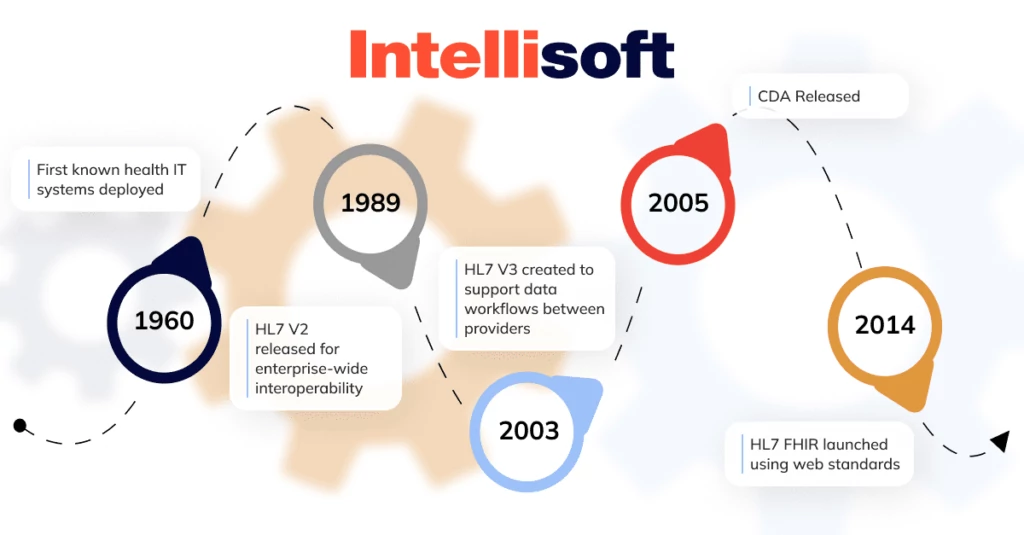
\includegraphics[width=1.0\textwidth]{Images/HL7_Versions.png}
            % \textbf{[Insert Figure Here: Evolution of HL7 Standards]}\\
            % \textit{Diagram illustrating the transition from V2 (Messaging) to V3 (RIM/Model) to FHIR (RESTful API/Resources).}
            % \vspace{2cm}
        \end{minipage}}
    \caption{Evolution of HL7 Standards from Messaging to RESTful Resources.}
    \label{fig:hl7_evolution}
\end{figure}

\section{Fast Healthcare Interoperability Resources (FHIR)}

In response to the complexity of HL7 v3 and the limitations of v2, HL7
introduced \textbf{FHIR} (Fast Healthcare Interoperability Resources) in 2012.
FHIR represents a paradigm shift from complex, custom healthcare protocols to
modern web standards.

\subsection{Core Architecture}
Unlike its predecessors, FHIR is built on the RESTful API approach widely used
in modern IT industries (e.g., by Google, Facebook, Twitter). It treats data
elements as independent "Resources"—modular components like \texttt{Patient},
\texttt{Observation}, or \texttt{Medication}—that can be accessed and
manipulated via standard HTTP methods (GET, POST, PUT, DELETE)
\cite{wiki_fhir}.

\subsection{Key Technical Advantages}
\begin{itemize}
    \item \textbf{Granularity via Resources:} FHIR allows systems to access specific data elements using unique URLs (e.g., \texttt{GET /Patient/123}), rather than exchanging entire heavy documents. This makes it ideal for mobile devices with limited bandwidth \cite{wiki_fhir}.

    \item \textbf{Modern Formats (JSON \& XML):} While previous standards relied on complex XML or pipe-delimited text, FHIR natively supports  JSON  (JavaScript Object Notation), which is lightweight and directly parsable by web browsers and mobile apps \cite{intellisoft}.

    \item \textbf{The 80/20 Rule:} FHIR focuses on defining the 20\% of requirements that satisfy 80\% of common healthcare use cases. For the remaining complex or local requirements, it uses a built-in extension mechanism, ensuring the core standard remains simple and implementable \cite{repo}.
\end{itemize}

\subsection{Comparison of Standards}
Table \ref{tab:comparison} highlights the fundamental differences between the
major HL7 standards, illustrating why FHIR was chosen as the interoperability
backbone for this project.

\begin{table}[ht]
    \centering
    \caption{Comparison of HL7 v2, v3, CDA, and FHIR Standards}
    \label{tab:comparison}
    \renewcommand{\arraystretch}{1.4}
    \begin{tabular}{|p{0.2\linewidth}|p{0.22\linewidth}|p{0.22\linewidth}|p{0.22\linewidth}|}
        \hline
        \textbf{Feature}          & \textbf{HL7 v2}                             & \textbf{HL7 v3 / CDA}                          & \textbf{FHIR}                                                      \\ \hline
        \textbf{Primary Paradigm} & \raggedright Event-Driven Messaging         & \raggedright Reference Model (RIM) / Documents & \raggedright RESTful API \& Resources \tabularnewline \hline
        \textbf{Data Format}      & \raggedright Pipe-delimited text            & \raggedright Complex XML                       & \raggedright JSON, XML, RDF \tabularnewline \hline
        \textbf{Transport}        & \raggedright LLP / MLLP (TCP/IP)            & \raggedright SOAP / Web Services               & \raggedright HTTP / REST \tabularnewline \hline
        \textbf{Complexity}       & \raggedright Moderate (Vague semantics)     & \raggedright High (Steep learning curve)       & \raggedright Low (Web-standard based) \tabularnewline \hline
        \textbf{Use Case}         & \raggedright Hospital Backend (ADT, Orders) & \raggedright Clinical Documents (Summaries)    & \raggedright Mobile, Web, Cloud, \& Backend \tabularnewline \hline
    \end{tabular}
\end{table}
\begin{figure}[H]
    \centering
    % REPLACE THE LINE ABOVE WITH YOUR ACTUAL IMAGE FILE
    \fbox{\begin{minipage}{0.7\textwidth}
            \centering
            % \vspace{2cm}
            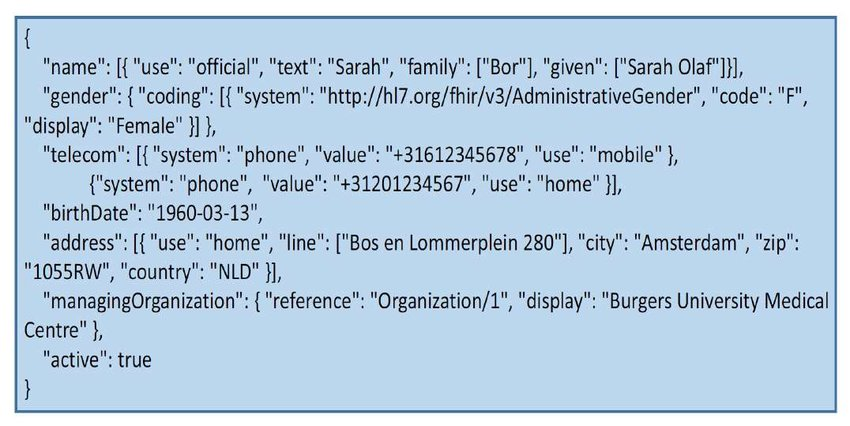
\includegraphics[width=1.0\textwidth]{Images/FHIR-patient-JSON-example-source-2.png}
            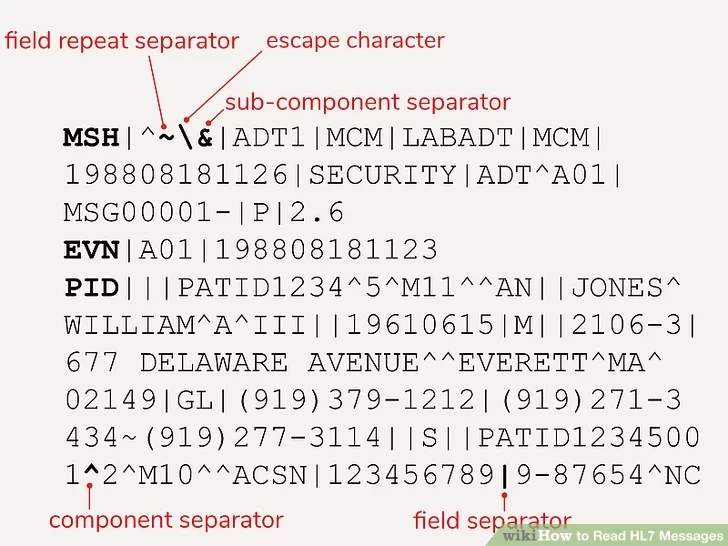
\includegraphics[width=1.0\textwidth]{Images/aid9705860-v4-728px-9705860-1.png}
            % \textbf{[Insert Figure Here: Structure of a FHIR Resource]}\\
            % \textit{Diagram showing a JSON snippet of a Patient Resource (Name, ID, Gender) vs. a legacy v2 Message string.}
            % \vspace{1cm}
        \end{minipage}}
    \caption{Visual Comparison of Data structure: HL7 v2 Message vs. FHIR JSON Resource.}
    \label{fig:fhir_structure}
\end{figure}

\section{Authentication and Authorization Standards}

\subsection{\ac{OAuth} 2.1 and OpenID Connect (OIDC)}
Modern web and mobile security paradigms have transitioned toward the \ac{OAuth} 2.1 consolidation framework, 
which deprecates inherently insecure vectors -such as the Resource Owner Password Credentials grant- due to the risks associated with client-side credential handling \cite{rfc6749}. 
The standard explicitly mandates the Authorization Code Flow combined with dynamic cryptographic extensions for native applications, and delegates browser session management to secure edge boundaries. 
OpenID Connect (OIDC) \cite{oidc} extends this framework by introducing an identity layer via ID tokens, enabling robust Single Sign-On (SSO) capabilities. 
Within decoupled health architectures, this project leverages gatekeeper abstractions to securely manage token translation scopes out-of-band.

\subsection{JSON Web Tokens (\ac{JWT})}
\ac{JWT}s \cite{rfc7519} are cryptographically signed structural tokens that encode user identity claims, access scopes, and session longevity attributes (e.g \texttt{iss}, \texttt{aud}, \texttt{exp}). 
Utilizing asymmetric signing algorithms (such as RS256) allows distributed microservices and backend API workers to perform stateless signature validation against an Identity Provider's JSON Web Key Sets (JWKS), 
removing the performance overhead of database lookups. 

\subsection{\ac{PKCE}}
\ac{PKCE} \cite{rfc7636} mitigates authorization code interception attacks on public and native clients by introducing a dynamic cryptographic secret exchange loop. 
By validating a high-entropy \texttt{code\_verifier} against a pre-computed \texttt{code\_challenge}, the protocol ensures that malicious actors tracking custom OS deep links cannot intercept or exchange leaked authorization codes for active token clusters \cite{rfc9700}.

\section{Healthcare Security and Integration Standards}

\subsection{\ac{FHIR} and \ac{SMART} on \ac{FHIR}} 
The \ac{FHIR} specification \cite{fhirhl7} provides structural consistency for healthcare models, 
but relies on external security profiles for transactional protection. 
The \ac{SMART} on \ac{FHIR} framework \cite{smart_fhir} addresses this by mapping \ac{OAuth} 2.0 access scopes directly to granular medical resources (e.g \texttt{patient/Observation.read}, \texttt{user/Condition.write}). 
This allows patient-controlled capability policies to interoperate seamlessly with standardized \ac{FHIR} Consent resource models \cite{fhir_consent}, enforcing time-bound, actor-specific boundaries directly over \ac{PHI}.

\section{Token-Based Architecture and Session Management}

\subsection{The Backend-for-Frontend (BFF) Pattern}
To guard web clients against \ac{XSS} token exfiltration, modern architectures employ the \ac{BFF} pattern \cite{draft_bff}. 
By containing OAuth token loops entirely behind an edge gateway, access and refresh tokens are kept out of reach of browser storage layers. 
The frontend-to-backend connection is secured via encrypted HTTP-only, Secure, and SameSite-restricted session cookies, preventing both script-based extraction and \ac{CSRF} vectors.

\subsection{Distributed Session State Cache}
While stateless JWT tokens simplify transaction execution, immediate security invalidation (e.g during logout) requires backchannel tracking. 
Utilizing low-latency, in-memory data structures (such as Redis) allows systems to maintain a real-time blacklist or session map, striking a secure balance between stateless processing speed and immediate session revocation capabilities.

\section{Edge Security and Infrastructure Defense}

\subsection{Perimeter Protection and Rate Limiting}
Securing electronic health records requires robust defenses at the ingestion boundary. 
Reverse proxies and API gateways (such as Nginx) isolate internal application nodes by terminating TLS profiles, dropping non-conforming HTTP payloads, and establishing strict rate-limiting boundaries backed by sliding-window token buckets to block distributed brute-force attempts and \ac{DoS} vectors \cite{ratelimit}.

\subsection{Mobile Application Isolation}
Native environments require a completely different security profile than web applications. 
Lacking standard cookie containment scopes, mobile applications mitigate malicious data access by isolating long-lived refresh tokens and active access JWTs inside hardware-backed storage containers, such as the Android Keystore \cite{android_keystore}, keeping secrets cryptographically secure even if the host operating system is compromised.

\section{Audit Logging, Diagnostics, and Forensic Compliance}

\subsection{Security Event Auditing}
Security tracing requires structured log recording for authentication lifecycles, user state transitions, data access denials, and cryptographic key rotations. 
To preserve forensic utility, processing engines must isolate audit trails in real time to automated storage pipelines to prevent accidental downstream data exposure \cite{owasp_logging}.


% \subsection{HIPAA and GDPR}
% HIPAA \cite{hipaa} requires access controls, 
% encryption (in transit/at rest), and audit logging for Protected Health Information. 
% GDPR \cite{gdpr} mandates data minimization, consent, and subject access rights.

